\section{Recursos principals del bloc Discussions}

    \paragraph{}
    El recurs principal d'aquest bloc de l'arbre familiar rep el nom de Discussió. Al mateix temps, podem dir que les discussions estan formades principalment per un conjunt de Comentaris.

    Les discussions a FamilySearch són tòpics de discussió introduïts pels usuaris i relacionats a una persona en concret. Com hem esmentat fa un moment, aquestes discussions estan formades per diferents comentaris i també destaca la utilització d'un recurs intermedi que fa de pont, entre les discussions i els recursos de les persones a les quals fan re\-fe\-rèn\-cia, mitjançant enllaços hypermedia.

    El contingut d'aquestes discussions és bastant divers, però generalment són u\-ti\-lit\-za\-des per discutir, entre diferents usuaris, sobre les dades relatives a una persona, l'origen de les fonts de dades i altres aspectes similars.

    La figura~\ref{img:discussionsBloc} mostra com es troben relacionats els recursos que conformen el bloc Discussions.

    \begin{figure}[h]
        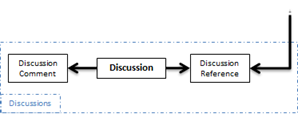
\includegraphics{05/05_discussionsCore}
        \centering
        \caption{El bloc de l'arbre familiar relatiu a les discussions}\label{img:discussionsBloc}
    \end{figure}

    Podreu observar també, a les taules que representen l'estructura dels recursos, que a vegades, per la columna que marca el format de dades d'un paràmetre, aquest es troba especificat entre els caràcters `[' i `]'. Aquesta terminologia s'utilitza per indicar que aquest paràmetre és en realitat un recurs o objecte de dades diferent inclòs dins del recurs estudiat.

    També s'observarà que sovint, els recursos exposats, hereten dades d'altres recursos i en els casos que aquests siguin rellevants, se n'exposarà l'estructura a l'apartat `Altres recursos interessants', més endavant en la memòria.

    \subsection{El recurs Referència a la Discussió (DiscussionsReference)}

    \paragraph{}
    Aquest recurs s'utilitza principalment perquè el recurs Persona puguin accedir al conjunt de discussions que tracten sobre ella i viceversa. En concret, existirà un enllaç per cada una de les discussions que reverenciïn a la mateixa persona.

    Les dades contingudes per aquest recurs poden ser trobades a la taula~\ref{res:discussionReference} i també hereta els paràmetres dels recursos Enllaços Hypermedia i Dades Extensibles que poden ser trobats a l'apartat `Altres recursos interessants'.

    \begin{center}
             \csvreader[
                separator=comma,
                before table=\sffamily\small,
                longtable={p{2cm-2\tabcolsep}p{3.5cm-2\tabcolsep}p{8.5cm-2\tabcolsep}},
                table head={\caption{Paràmetres del recurs Referència a la Discussió}\label{res:discussionReference}\\\toprule%
                    \headentry{m{2cm-2\tabcolsep}}{Paràmetre}
                    & \headentry{m{3.4cm-2\tabcolsep}}{Format de Dades}
                    & \headentry{m{8.5cm-2\tabcolsep}}{Descripció}\\\midrule},
                late after line=\\\midrule,
                late after last line=\\\bottomrule,
             ]
             {./tables/05/03_discussions/discussionReference.csv}
             {param=\param,format=\format,desc=\desc}
             {\param&\format&\desc}
     \end{center}

    \subsection{El recurs Discussió (Discussion)}

    \paragraph{}
    El recurs Discussió és utilitzat per representar el tòpic sobre el qual tractarà la conversació entre els diferents usuaris de FamilySearch i emmagatzemar el conjunt de comentaris introduïts per aquests.

    El recurs Discussió, esdevé un objecte bastant simple, contenint només la informació necessària perquè altres usuaris puguin comprendre el tòpic de discussió, les metadades de la creació i accedir al conjunt de comentaris.

    Aquest recurs està format pels paràmetres mostrats a la taula~\ref{res:discussion} i també hereta els paràmetres dels recursos Enllaços Hypermedia i Dades Extensibles, que poden ser trobats a l'apartat `Altres recursos interessants'.

    \begin{center}
             \csvreader[
                separator=semicolon,
                before table=\sffamily\small,
                longtable={p{2cm-2\tabcolsep}p{3.5cm-2\tabcolsep}p{8.5cm-2\tabcolsep}},
                table head={\caption{Paràmetres del recurs Discussió}\label{res:discussion}\\\toprule%
                    \headentry{m{2cm-2\tabcolsep}}{Paràmetre}
                    & \headentry{m{3.4cm-2\tabcolsep}}{Format de Dades}
                    & \headentry{m{8.5cm-2\tabcolsep}}{Descripció}\\\midrule},
                late after line=\\\midrule,
                late after last line=\\\bottomrule,
             ]
             {./tables/05/03_discussions/discussion.csv}
             {param=\param,format=\format,desc=\desc}
             {\param&\format&\desc}
     \end{center}

    \subsection{El recurs Comentari (Comment)}

    \paragraph{}
    El recurs Comentari conté els missatges introduïts pels diferents usuaris com a resposta a una discussió. Principalment, conté informació sobre la data de creació, l'usuari que l'ha enviat i el text en qüestió propi del comentari.

    Les dades pròpies d'aquest recurs es mostren a la taula~\ref{res:comment} i també hereta els paràmetres dels recursos Enllaços Hypermedia i Dades Extensibles que poden ser trobats a l'apartat `Altres recursos interessants'.

    \begin{center}
             \csvreader[
                separator=comma,
                before table=\sffamily\small,
                longtable={p{2cm-2\tabcolsep}p{3.5cm-2\tabcolsep}p{8.5cm-2\tabcolsep}},
                table head={\caption{Paràmetres del recurs Comentari}\label{res:comment}\\\toprule%
                    \headentry{m{2cm-2\tabcolsep}}{Paràmetre}
                    & \headentry{m{3.4cm-2\tabcolsep}}{Format de Dades}
                    & \headentry{m{8.5cm-2\tabcolsep}}{Descripció}\\\midrule},
                late after line=\\\midrule,
                late after last line=\\\bottomrule,
             ]
             {./tables/05/03_discussions/comment.csv}
             {param=\param,format=\format,desc=\desc}
             {\param&\format&\desc}
     \end{center}

